


%%%%%%%%%%%%%%%%%%%%%%%%%%%%%%%%%%%%%%%%%
% Journal Article
% LaTeX Template
% Version 2.0 (February 7, 2023)
%
% This template originates from:
% https://www.LaTeXTemplates.com
%
% Author:
% Vel (vel@latextemplates.com)
%
% License:
% CC BY-NC-SA 4.0 (https://creativecommons.org/licenses/by-nc-sa/4.0/)
%
% NOTE: The bibliography needs to be compiled using the biber engine.
%
%%%%%%%%%%%%%%%%%%%%%%%%%%%%%%%%%%%%%%%%%

%----------------------------------------------------------------------------------------
%	PACKAGES AND OTHER DOCUMENT CONFIGURATIONS
%----------------------------------------------------------------------------------------

\documentclass[
	a4paper, % Paper size, use either a4paper or letterpaper
	10pt, % Default font size, can also use 11pt or 12pt, although this is not recommended
	unnumberedsections, % Comment to enable section numbering
	twoside, % Two side traditional mode where headers and footers change between odd and even pages, comment this option to make them fixed
]{LTJournalArticle}


\newcommand{\A}{{\cal A}}
\newcommand{\R}{\mathbb R}
\newcommand{\Z}{\mathbb Z}
\newcommand{\Q}{\mathbb Q}
\newcommand{\N}{\mathbb N}
\newcommand{\C}{\mathbb{C}}
\newcommand{\PP}{\mathbb{P}}
\newcommand{\E}{\mathbb{E}}
\newcommand{\sig}{\sigma \text{-algebra}}
\newcommand{\1}{\mathbbm{1}}


\newcommand\invisiblesection[1]{%
  \refstepcounter{section}%
  \addcontentsline{toc}{section}{\protect\numberline{\thesection}#1}%
  \sectionmark{#1}}

\usepackage{appendix}
\usepackage{comment}
\usepackage{mathtools}
\usepackage{multicol}
\usepackage{hyperref}
\usepackage{url}
\usepackage{amssymb}
\usepackage{amsmath}
\usepackage{amsmath, amsthm, amssymb, url, hyperref}


\usepackage{hyperref}
\hypersetup{
    colorlinks=true,
    linkcolor=blue,
    filecolor=magenta,      
    urlcolor=cyan,
    pdftitle={Overleaf Example},
    pdfpagemode=FullScreen,
    }

\urlstyle{same}

\DeclareMathOperator*{\argmin}{arg\,min}

\usepackage{fancyvrb}


\usepackage{algorithm}

\newtheorem{theorem}{Theorem}
\newtheorem{corollary}{Corollary}[theorem]

%\usepackage[T1]{fontenc}
%\usepackage{babel}
%\usepackage{csquotes}
%\usepackage{biblatex}



%\usepackage{biblatex}
\usepackage[american]{babel}
\usepackage{csquotes}
\usepackage[backend=biber]{biblatex}
\DeclareNameAlias{author}{last-first}
\addbibresource{mybib.bib} % BibLaTeX bibliography file







\runninghead{STAT 447C Project} % A shortened article title to appear in the running head, leave this command empty for no running head

\footertext{\textit{Department of Statistics, The University of British Columbia}} % Text to appear in the footer, leave this command empty for no footer text

\setcounter{page}{1} % The page number of the first page, set this to a higher number if the article is to be part of an issue or larger work

%----------------------------------------------------------------------------------------
%	TITLE SECTION
%----------------------------------------------------------------------------------------

\title{Comparing Methods: Naïve Elastic Net against Bayesian Regression with a Horseshoe Prior} % Article title, use manual lines breaks (\\) to beautify the layout

% Authors are listed in a comma-separated list with superscript numbers indicating affiliations
% \thanks{} is used for any text that should be placed in a footnote on the first page, such as the corresponding author's email, journal acceptance dates, a copyright/license notice, keywords, etc
\author{Sarah Masri \\ 97415681}

% Affiliations are output in the \date{} command
\date{\textsuperscript{STAT 447C} \\
\textsuperscript{The University of British Columbia} \\ 
\textsuperscript{April 19, 2023} }

% Full-width abstract
\renewcommand{\maketitlehookd}{%
	\begin{abstract}
\noindent Large-scale epigenetic analyses are an increasingly useful tool for prognostic prediction of disease and associated gene activation \cite{Tang2017}. Problems involving high-dimensional gene expression data are often challenging by nature due the number of predictors being much larger than the number of observations. Regularized mechanisms with built-in variable selection are often employed to overcome this. The objective of this project is to compare performance and advantages of some regularized linear regression approaches to Bayesian hierarchical generalized linear models in high-dimensional inference. Namely, to compare elastic net regression to Bayesian penalized regression with a horseshoe prior in the context of prediction and gene detection for high-dimensional molecular data. 
\\
\\
A public repository containing implemented methodology can be found through this \href{https://github.com/sarahmasri/stat447C-Project}{this link}.
	\end{abstract}
}

%----------------------------------------------------------------------------------------

\begin{document}

\maketitle % Output the title section

%----------------------------------------------------------------------------------------
%	ARTICLE CONTENTS
%----------------------------------------------------------------------------------------

\section{Introduction}
% - Problem formulation. (15%) The report clearly describes:
%       - a real-world inference task/problem,
% succinct but sufficient context (e.g. biological terminology) needed to understand the problem,
%       - the key modelling/methodological/challenge, clearly associating it with one of the items under “menu of project themes” above.


% - Regularized regression with a sparsity inducing penality (LASSO, EN, SCAD) = common approach to feature selection for building predictive models based on high-diensional data, and can be effectively used for a joing analysis of multi-omic profiles measured on the same sample


The host immune response is an incredibly complex system responsible for eliminating pathogens (e.g., viruses, bacteria) to protect the organism from infection or disease. Studying this functionality is crucial to understanding how an organism defends itself against foreign invaders, and helps incite progress over a variety of applications such as vaccine development, treatment for infectious disease, advancing cancer immunotherapy, and stimulating general improvements in healthcare and disease prevention \cite{noauthor_undated}. 

The host immune response is made up of a myriad of cell types that vary in biological properties and physical location. Specifically, the immune system is comprised of two parts the work together but perform different tasks: the more general innate immune system, and the specialized adaptive immune system \cite{noauthor_2020}. Innate immune cells such as eosinophils, neutrophils, basophils, monocytes, and mast cells, are a hosts first line of defense against pathogens. Adaptive immune cells such as B lymphocytes and T lymphocytes are responsible for identifying different antigens. The innate and adaptive systems are linked through Natural Killer cells and antigen presenting cells, such as macrophages \cite{Torang2019}. 

Recent technological advancements such as mass cytometry and single-cell RNA sequencing (scRNA-seq), have progressed in the pursuit of differentiating between immune cell subsets in transcriptomics data (RNA expression data) with increasing accuracy \cite{Lin2022}. However, this kind of genomic data  presents challenges due to its high-dimensional nature, often with a much larger number of predictors than samples as well as noisy and missing values. Machine learning methods are an accessible way to address these challenges by selecting gene subsets and estimating gene coefficients through regression models simultaneously. This can be done through a frequentist of Bayesian lens, using a variety of methods. 

This report aims to compare the accuracy and efficiency of the frequentist naïve elastic net regression against the horseshoe prior for Bayesian regression for selecting gene subsets and estimating gene coefficients. A review of historical literature and methodoloy related to this comparison is provided, followed by a methodological description for each model, and finally a comparison carried out on real transcriptomic data. 




\subsection{Literature Review}

In both research and industry, it is not uncommon to encounter high-dimensional datasets with a much larger number of predictors than samples, such as in gene expression data \cite{Narisetty2020}. Including all covariates in such a dataset may lead to overfitting, and so determining which covariates are relevant to the outcome of interest becomes an increasingly useful problem. This can be accomplished through methods that perform model selection through either a frequentist of Bayesian framework. The comparison of frequentist against Bayesian methods is not a novel contrast, but an important one. When formulating a problem, it is crucial to choose methods that achieve the greatest possible accuracy and computational efficiency. 

This report restricts its methods to high-dimensional gene expression data. Although the application of the results is unique, the comparison of methods may be extended to other fields and applications that require similar high-dimensional datasets. Hence, this literature review includes the comparison of penalized linear regression models to comparable Bayesian approaches on high-dimensional data rather than the gene-expression data, although much of the literature cited is within the application of genomics.


A commonality between frequentist and Bayesian methods for gene selection and the estimation of gene coefficients is the application of shrinkage methods. Each of these methods pursue an optimal trade-off between accuracy and computational efficiency. These literature includes applications of the frequentist penalized regression methods assessed on their own, or compared directly against Bayesian priors with shrinkage properties. Some papers extend this comparison into novels approaches combining frequentist and Bayesian methods. 


Narisetty (2020) provides a comprehensive review and comparison of some of the most well-known methods for variable selection on high-dimensional data. Both frequentist and Bayesian methods are included, with an emphasis on Bayesian approaches with priors that induce shrinkage and sparsity. Frequentist methods include LASSO, elastic net, adaptive least-squares methods, and other regression methods with a nonconvex penalty. Bayesian frameworks for model selection are reviewed including a spike and slab prior, a horseshoe prior, global-local shrinkage priors, and a review of Gibbs sampling to compute the posterior distribution. Other samplings and approximation algorithms are reviewed (e.g., Laplace approximation, variational approximation). A variety of these widely used models are implemented on polymerase chain reaction (PCR) data, with results indicating Bayesian methods yielding better performance (smaller BIC) when compared to other frequentist methods. Namely, LASSO regression returns a model size of 10 and BIC of 144.22 whereas a Bayesian implementation with a horseshoe prior returns a model size of 7 with a BIC of 126.54. 


More frequentist penalized regression methods are explored in Waldmann et al. (2013), Torang et al. (2019), and Ogutu et al. (2012). Linear regression methods with convex penalties including LASSO and elastic net are shown to overcome some challenges from high dimensional data through their shrinkage properties and selection operators. Cross validated results on simulated and real world data show optimistic results for lasso and elastic net. Namely, these methods used as classifiers for genomic selection returned greater accuracy compared to ride regression and non-regularized linear regression models. 


Outside of the frequentist school of thought, Bayesian estimation using a horseshoe prior on high-dimensional data is propose in Banerjee (2022). This choice is motivated by the ability of the horseshoe prior to induce a strong shrinkage effect on the mean parameters. The estimation performance is demonstrated on both simulated and real-life data, returning results with particularly high accuracy, precision, and sensitivity. 


Münch et al. (2021) implements an adaptive group-regularized logistic elastic net regression method on both simulated and RNAseq data. This paper highlights the common criticism of elastic net, that feature selection is often unstable and returns different features for different instances of the data. Including prior information to the model seems to reduce this instability, and refers to a possible benefit of extending the method to a group-regularized horseshoe model. Other combined methods are proposed in Li and Lin (2010), and Makalic and Schmidt (2015). It is shown that a Bayesian elastic net behaves comparably with a non-Bayesian elastic net, but better in feature select \cite{Li2010}. Additionally, a Bayesian horseshoe linear regression outperforms other Bayesian methods in terms of computational efficient for high-dimensional data. 

Finally, Bhadra et al. (2017) contrast and surveys the Lasso and horseshoe regularization on high-dimensional data. the paper discusses the theoretical optimality for both Lasso and horseshoe estimators, and notes how horseshoe regression has not been studied at the same depth of penalized regression. It is addressed that the theoretical optimality of these methods rely on the underlying assumptions of the data. The paper concluded with optimism towards the Bayesian horseshoe estimator. 

Although Bhadra et al. (2017) compared a penalized least-squares method with horseshoe regression, no papers found compared a naïve elastic net directly against the Bayesian horseshoe. This report aims to extend the result of this literature to the use of such methods on high-dimensional transcriptomics data. 



\begin{comment}



\cite{Bhadra2017}
- LASSO vs horseshoe
- theoretical optimality in high-dimensional inference
- efficiency and scalability
- methodological development and performance
- also review Bayesian Lasso and EN


\end{comment}

\section{Methods}
% - Data analysis (40%)
%        - A Bayesian model is precisely described (e.g. using the .. ~ .. notation)
%         - Implementation code in the appendix (e.g. using Stan)
%         - Prior choice is motivated. If appropriate, several choices are compared or sensitivity analysis is performed.
%         - Critical evaluation of the posterior approximation. An appropriate combination of diagnostics, synthetic datasets and other validation strategies.

\subsection{Naïve Elastic Net Regression}
% - The report contains a literature review: (10%) relevant literature is cited and properly summarized.

Regularized methods for linear regression have the ability to control the complexity of a linear regression model by penalizing coefficients and effectively performing model selection. This is commonly used for feature selection on high-dimensional data and can be particularly useful for genomic data. Elastic net regression, a method within the family or regularized regression methods, is a hybrid model that combines an $L_1$ and $L_2$ penalty to shrink coefficients of predictors. The emergence of this method was due to lasting critique of LASSO regression, that it's feature selection is too dependant on the data itself which may lead to unstable results \cite{Zou2005}. This combination of penalties helps to reduce the possibility of overfitting and adjust for collinearity, and has been shown to outperform other regularized methods such as LASSO and Ridge regression in very high dimnsional data \cite{Torang2019, Zou2005}. 

Consider a data set with $n$ observations and $p$ predicts. Let ${\bf X} = ({\bf x}_1 | \ldots | {\bf x}_p) \in \R^{n \times p}$ represent the design matrix and ${\bf y} \in \R^n$ be the response. Assume that the response is centered and predictors are standardized such that,
\begin{equation}
\label{eq:EN-assume}
\sum_{i=1}^n y_i = 0, \hspace{5mm}
 \sum_{i=1}^n x_{ij} = 0, \hspace{5mm} 
 \text{and, } 
 \sum_{i=1}^n x_{ij}^2 = 1,
 \end{equation}
for $j = 1, 2, \ldots, p$. For some non-negative hyper-parameters, the naïve elastic net (NEN) loss function is defined as
\begin{equation}
    \label{eq:EN-loss}
    L(\lambda_1, \lambda_2, \beta) = \|{\bf y} - {\bf X} \beta\|_2^2 + \lambda_1 \|\beta\|_1 + \lambda_2 \|\beta\|^2_2.
\end{equation}


\noindent This function can also be generalized to 
\begin{equation}
\label{eq::EN-alt}
     L(\lambda, \alpha, \beta) = \|{\bf y} - {\bf X} \beta\|_2^2 + \lambda (\alpha \|\beta\|_1 + (1- \alpha) \|\beta\|^2_2),
\end{equation}
\noindent for some $\alpha \in [0, 1]$. If $\alpha=0$, the penalty term is reduced to that of LASSO regression, and if $\alpha=1$ it is reduced to the penalty of ridge regression. The NEN estimator $\hat{\beta}$ is the minimize of it's loss function defined by,

\begin{equation}
\label{eq:EN}
    \hat{\beta} = \argmin_\beta L(\lambda_1, \lambda_2, \beta). 
\end{equation}


In short, NEN can be considered as a penalized least squares problem. The solution to the NEN problem can be shown through simple algebra by transforming the problem into an equivalent LASSO problem by augmenting the data \cite{Zou2005}. Given ${\bf y}$ and  ${\bf X}$, define ${\bf y}^* \in \R^{n+p}$, ${\bf X}^* \in \R^{(n+p \times p)}$ such that
\begin{equation}
    {\bf y}^* = \begin{pmatrix}
        {\bf y} \\ {\bf 0}_p
    \end{pmatrix}, \hspace{5mm}
    {\bf X}^* =(1 + \lambda_2)^{-1/2} \begin{pmatrix}
        {\bf X} \\ \sqrt{\lambda_2} \ {\bf I}_{p \times p}
    \end{pmatrix}
\end{equation}

\noindent Let $\gamma = \frac{\lambda_1}{\sqrt{1 + \lambda_2}}$ and $\beta^* = \sqrt{1 + \lambda_2} \beta$. We can write the NEN loss function as 
\begin{equation}
    L(\gamma, \beta^*) = \|{\bf y}^* - {\bf X}^* \beta^*\|_2^2 + \gamma \|\beta^*\|_1.
\end{equation}


\noindent Further, let
\begin{equation}
\label{eq:EN-star}
    \hat{\beta}^* = \argmin_{\beta^*} L(\gamma, \beta^*). 
\end{equation}

\noindent Finally, we get
\begin{equation}
    \hat \beta = \frac{1}{\sqrt{1 + \lambda_2}} \beta^*.
\end{equation}



The tuning parameters $(\lambda, \alpha)$ control the strength and trade-off between the $L_1$ and $L_2$ penalties. A smaller value of $\lambda$ leads to stronger regularization and more sparse coefficient estimates. The $L_1$-ratio parameter $\alpha$ determines the ration of $L_1$ and $L_2$ penalties. Cross-validation methods like grid search can help optimize these hyperparameters for model performance, and adjust uniquely to the dataset being used to build the model.  

% ANALYTIC SOLUTION

%To solve such a problem computationally, one may choose to use coordinate descent, an optimization algorithm often used to minimize the loss function of a given model. The algorithm works by iteratively updating the regression coefficient until convergence.  


\begin{comment}
In each iteration of the algorithm, the optimization step may be expressed as described by Allerbo et al.,
\begin{equation}
    \hat{\beta} (t + \Delta t) = \hat \beta (t) - \Delta t \cdot \Delta \hat \beta.
\end{equation}    
\end{comment}


%- during gradiaent descent optimizatin of its cost function - L-2 penalty term = lowers weights to zero
%- then hypothesis gets sim pler and more gneal - less prone to overfitting
%- L2 shrinks weights close to zero = eliminates features present in hypothetical function = encourages sparsity

\subsection{Horseshoe Prior}

The horseshoe prior is a Bayesian prior distribution with strong theoretical guarantees in the context of regression analysis. The motivation behind the hoice of this prior is largely due to its shrinkage properties, the ability to identify true non-zero coefficients, which is particularly useful for datasets with a large number of predictors and small number of samples. The tails of this distribution is rather wide and decays like a second-order polynomial. It follows that it's penalty functions exhibits logarithmic behaviour, and is non-convex \cite{Bhadra2017, Banerjee2022}.

The horseshoe prior for regression coefficients $\beta \in \R^p$, with some global shrinkage parameter $\tau$, is given by the normal means model integrated into the following hierarchicial model,
\begin{align*}
    {\bf y}  |  {\bf X}, \beta  &\sim \mathcal{N}( {\bf X} \beta , \sigma^2  {\bf I_n}), \\
    \beta_i | \lambda_i^2, \tau^2, \sigma^2 &\sim \mathcal{N}(0, \lambda_i^2 \tau^2 \sigma^2),\\
    \sigma^2 &\sim \sigma^{-2} d \sigma^2, \\
    \lambda_i^2| \nu_i &\sim  \mathcal{IG}(1/2, 1/\nu_i), \\
    \tau^2 | \zeta &\sim \mathcal{IG}(1/2, 1/\zeta), \\
    \nu_1, \ldots, \nu_p, \zeta &\sim \mathcal{IG}(1/2, 1)
\end{align*}

\noindent for $i = 1, 2, \ldots, p$ \cite{Bhadra2017}. Note that the above makes use of the scale mixture representation of the half Cauchy distribution \cite{Banerjee2022}. Specifically, for some half Cauchy random variable $X \sim C^+(0, \psi)$ , we can write 
\begin{equation}
    X^2 | \phi \sim \mathcal{IG}(1/2, 1/\phi), \hspace{5mm} \phi | \psi \sim \mathcal{IG} (1/2, 1/\psi^2)
\end{equation}
\noindent where $\mathcal{IG}(\cdot , \cdot)$ denotes the inverse gamma distribution. 

The hierarchical models allows for the convenient use of a Gibbs sampling scheme to sample the posterior distribution \cite{Makalic2016}. Makalic and Schmidt (2016) give posterior distributions of the regression coefficients $\beta$, $\sigma^2$, the local and global hyper-variances $\lambda_j^2$ and $\tau^2$, and the auxiliary variables $\nu_j$ and $\zeta$.  As seen in equations \eqref{eq:A1} - \eqref{eq:A6}, the conditional posterior distributions for all parameters except $\beta$ follow an inverse-Gamma distributions. 



% add pictures?
\begin{comment}
Bhadra2017
- continuous shrinkage rule for sparse signal recovery
- motivation: normal means model
\end{comment}

\subsection{Data}

The elastic net method compared against a Bayesian regression model with a horseshoe prior is performed on real-world transcriptomics data. This data include 175 immune cells sequenced from 11 patients diagnosed with breast cancer \cite{Chung2017}. The data is taken from the Gene Expression Omnibus, which is a public data repository for array and sequence-based genetic data \cite{Edgar2002}. Data cleaning, pre-processing, and normalization protocols are sourced from Torang et al., (2019). 

The data consists of RNA sequenced data from 15 different immune cell types. These cell types are inherently divided into two groups: immune cells and adaptive cells. If these cell types were to be analyzed together, then any method applied may unnecessarily eliminate genes due to gene overlap between groups \cite{Torang2019}. To avoid this issue, only immune cells are analysed in this report. Finally, there are 15453 total genes (covariates) observed in the dataset. 





\begin{comment}
- verification dataset: scRNA-seq data derived from CD45+ cell samples from breast cancer with GEO accession numbers GSE75688
= data normalization: instead of using raw data to develop individual gene signatures and cell classification models, they implemented a multistep normalization process before training models
- eliminated obviously insignificant genes from the data - kept genes with expressions values >= 5 counts in at least 5 samples for immune cell samples
- for T helper samples only >= 5 counts was needed since few of these samples were present in the data
- the completed main normalization step (withinLaneNormalization and betweenLaneNormalization from EDASeq package in R_ to remove GC-content biases 
- after normalization, filteration

- missing values: imputation method on missing values - not mean imputation - set a dummy constant instead since mean imputation was not meaningful

\end{comment}


\subsection{Analysis}

The primary goal of the analysis is to train a gene selection model on immune cell types. Genetic data often requires extensive pre-processing that is motivated primarily by the underlying biology and not the statistical methods intended for use. The pre-preprocessing used for this data is borrowed from Torang et al. (2019) and is not unique to the methods used in this report. First, the data is adjusted using a multistep normalization process before training the models. Then, insignificant genes will low expression counts are removed from the dataset. Finally, missing values are imputed.

The dataset is split into training and testing sets of size 108 and 77 respectively. A cross-validated elastic net model to performer gene selection and coefficient estimation is fit on the training set using \verb|cv.glmnet| with \verb|nfold=10| from the \verb|glmnet| package in \verb|R|. This minimizes the loss defined by equation \ref{eq::EN-alt} for each $\lambda = 0.1, 0.05, 0.01, 0.005, 0.001, 0.0005, 0.0001$. 

Additionally, Bayesian regression with a horseshoe prior as described above is implemented on the training set to select genes and estimate gene coefficients. The probabilistic programming language is employed using the \verb|RStan| package to fit the specified model to the data using Markov Chain Monte Carlo (MCMC) sampling with 2000 iterations and 4 chains. This process allows for Bayesian estimation of regression coefficients while incorporating the horseshoe prior, which promotes sparsity in the coefficient estimates. 

Note that Torang et al., (2019) simulated supplementary noisy data using the limited transcriptomics data available. This was not possible for the purposes of this report, since estimating models from this much larger dataset is too computationally burdensome to compute on the machine used during this analysis. The limited number of genetic samples are analysed, with the expectation of low performance. 



\begin{comment}
- also analyzed a second dataset that included 317 epithelial breast cancer cells, 175 immune cells, and 23 non-carcinoma stromal cells from 11 patiens diagnosed with BC
- only considered samples annotated as immune cells
- used proposed classifier
\end{comment}

\section{Results}


\subsection{Simulation}

Since the breast cancer data is not expected to demonstrate the methods described to their full potential, a much simpler dataset is simulated to compare methods. Synthetic data is simulated following a linear regression model
\begin{equation}
    \label{eq:regression}
    {\bf y} =  {\bf X} \beta + \varepsilon
\end{equation}
\noindent where $ {\bf y} \in \R^n$ is the response, $ {\bf X} \in \R^{n\times p}$ is the design matrix, $\beta$ is the vector of true regression coefficients, and $\varepsilon$ is the random error term assumed to follow a Normal distribution. The number of samples are fixed to be $1000$, and the number of predicts $100$. To generate ${\bf X}$, values are randomly drawn from a standard Normal distribution. Predictors are also normalized to have mean zero and unit variance to ensure they exist on the same scale. True regression coefficients $\beta$ are represented by a sparse vector, with 7 non-zero coefficients sampled uniformly at random in the interval $(-5, 5)$. This simulates the circumstance where only a few predictors influence the response variable. Finally, ${\bf y}$ is computed using equation \ref{eq:regression}. 

Naïve elastic net is fitted using a logarithmic grid of 100 proposed values of $\lambda$ in the interval $(0.001, 1000)$. An approximate optimal value of $\lambda=0.0376$ is selected by minimizing the cross-validated mean square error over. A mixing parameter of $0.05$ is selected to establish an equal balance between $L_1$ and $L_2$ penalties. A visualization of this choice can be observed in Figure \ref{fig:EN-lambda}.

\begin{figure}[ht] %{figure*}[ht!]
\centering
\captionsetup{justification=centering, margin=-0.2cm}
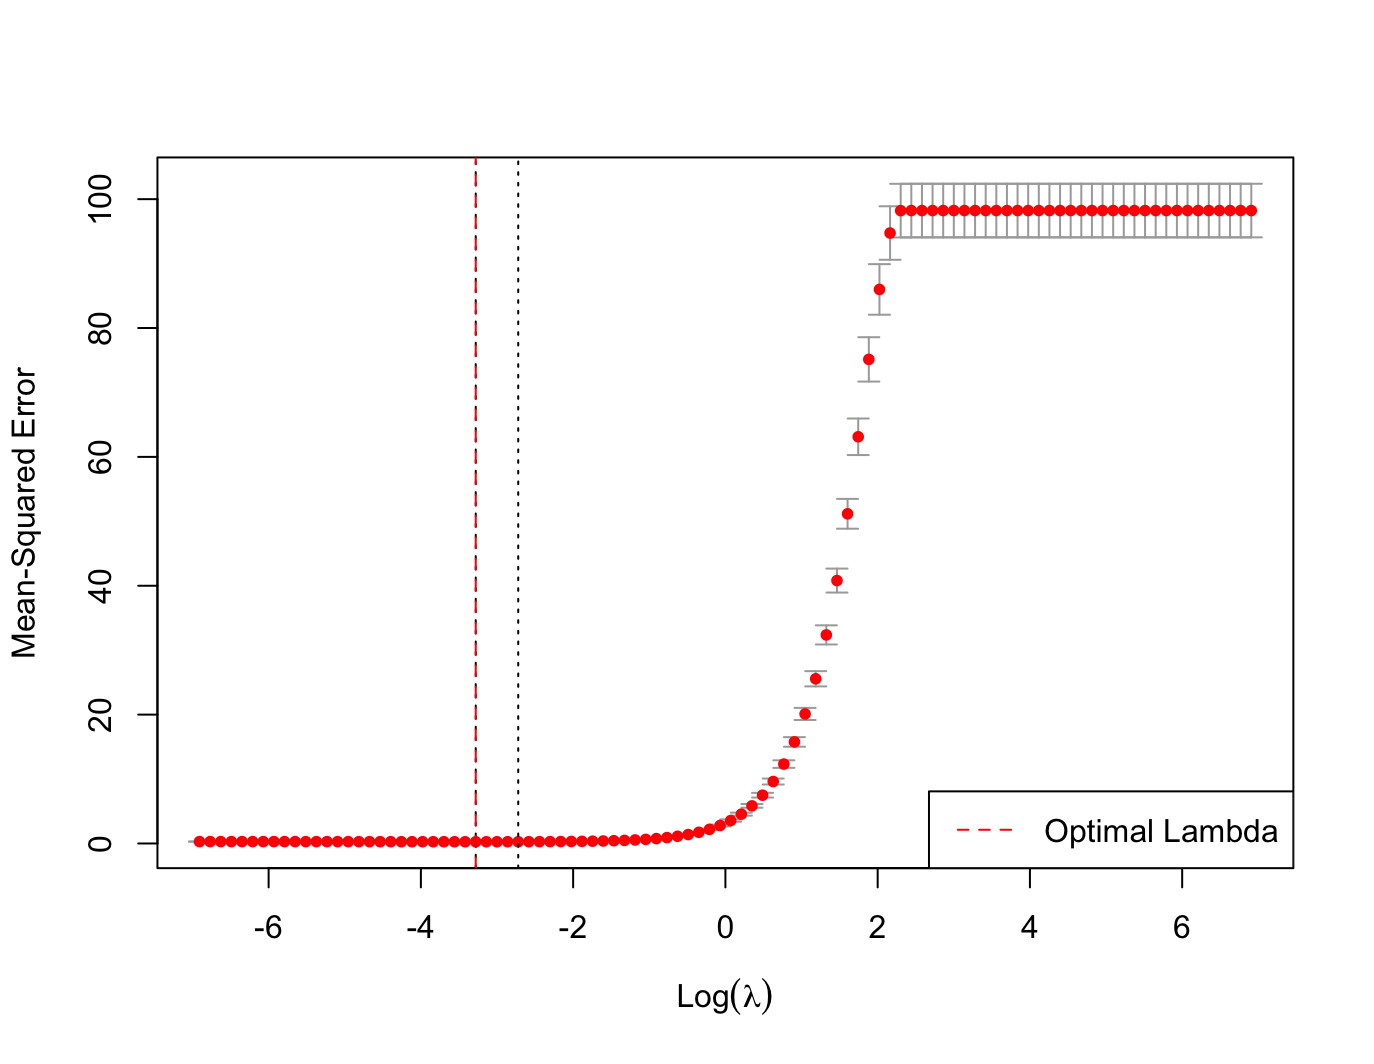
\includegraphics[width=0.4\textwidth]{Figures/simulate_lambda.png} 
\caption{\textbf{Simulation Optimal Lambda} \\
Cross-validated errors over different values of $\lambda$ computed in the naïve elastic net model. Vertical dashed lines indicate the most optimal values selected via cross validation.}
\label{fig:EN-lambda}
\end{figure} 

Bayesian regression with a horseshoe prior is subsequently. As discussed previously, this introduces a hierarchical model where the regression coefficients $\beta$ are assumed to follow a sparse prior distribution. This methodology encourages sparsity by allowing some coefficients to shrink to zero, which is indeed observed in the results. Since only 2000 iterations per chain are run, variable selection is performed with a threshold of 0.001. In other words, regression coefficients less than 0.001 are assumed to be shrunken to zero, and not needed in the regression model. 


\begin{table}[!htbp]
\centering
\caption{\textbf{Fitted Model Results}}
\label{tab:results}
\begin{threeparttable}
\begin{tabular}{p{3.5cm}p{1cm}p{1.5cm}}
\toprule
 & {\bf NEN} & {\bf Horseshoe} \\ 
  \hline
 {\bf MSE} & 0.236  & 0.240 \\
 {\bf Number of Selected Variables} & 34 & 28 \\
 {\bf Number of Correctly Selected Variables} & 2 & 3  \\
   \hline
\bottomrule
\end{tabular}
\end{threeparttable}
\caption*{Table reporting results from fitted NEN and horseshoe}
\end{table}


Results from the simulated data show that the NEN and Bayesian regression model with a horseshoe prior perform comparably, the NEN reporting a lower and more desirable mean square error (MSE), but the horseshoe model return more sparse coefficients, closer to the ground truth.


\subsection{Breast Cancer Data}

The NEN and horseshoe methods were each applied on the high-dimensional breast cancer data. Cell types are classified through each model, and non-zero gene coefficients are returned. It is important to note that despite the limited data, the NEN method took approximately 40 seconds to run and the Bayesian regression with a horseshoe prior took over 12 hours. The latter computational length might be explained by the high dimensional of the dataset, and the complexity of the horseshoe prior. It is possible that a more simple prior that involves fewer hyperparameters may have been less computationally demanding. 

%write which lambda min

As expected, results from NEN reflect a poor fit. With an optimal $\lambda = 0.0001$, the total cell type classification accuracy is reported to be only 0.365. The generated breast cancer data used in Torang et al. (2019)'s study reflect classification of approximately 0.876 indicating that our poor performance is likely due to the extremely small number of samples compared to the much larger number of predictors. It is important to note that the focus of this report is no to classify cell type, but to examine the feature selection capabilities between the two methods since our \verb|stan| code is not adapted to perform classification. 

NEN selects a total of 110 genes to be used in the regression model out of a total 1946 genes, whereas Bayesian regression with a horseshoe prior selects 1946 that are far from zero. The use of the term "far from zero" reflects a gene coefficient threshold of 0.1. In other words, since only 2000 iterations were used for each chain in the MCMC algorithm, coefficients with absolute value less than or equal to 0.1 are assumed to be close enough to 0 to exclude from the regression model. It is notable that each model captured a unique different subset of genes, with no intersection. It is not possible to validate the accuracy these coefficients since determining the true gene expression scores with absolute certainty is challenging biologically, and no ground truths are provided in the dataset. 

The stark differences in the selected genes may provide insight to the biological factors underlying this data. NEN tends to favour features that demonstrate strong linear relationships with the response, implying that its selected genes exhibit strong linear dependencies in the dataset. Alternately, Bayesian regression with a horseshoe prior assumes the gene coefficients to be close to zero, but allows for a small subset of coefficients to be large. Instead of capturing linear relationships, this method instead reflects significant non-linear or sparse associations within the dataset. Overall, these difference in selected genes may be explained by the complicated nature and diversity of genomics data, and highlights the importance of employing multiple statistical techniques. 











\begin{comment}
    - we classified each cell type and counted the number of true predictions for each method
    - visaluze perfomance of different lambdas by generating True-Negative samples using a bootstrapping approach - synthetic data (I didn't do this)
    - generate ROC curves and AUC used to score each lambda value
    - inflection point at lambda vlaue = 0.05 - adding additional genes by increasing lambda reduced AUC (72 genes?_
    - coefficients also correlated with expression levels - heatmas
\end{comment}



\section{Conclusion}

Although the results from the breast cancer data is not as informative as one would hope in a formal study, the completion return of the implementation offer optimism in utilizing Bayesian regression with a horseshoe prior on this kind of genomic data. The differences in performance and results of these methods underscores the importance of applying diverse methodology within this field. Both NEN and Bayesian regression with a horseshoe prior extract meaningful insights into transcriptomics, their methods are built on incomparable foundations, with NEN emphasizing linear relationships, and Bayesian regression prioritizing sparse signal detection and non-linear associations. B leveraging the strengths and differences between these kinds of frequentist against Bayesian methods towards feature selection and coefficient estimation, researchers can gain a broader, more comprehensive understanding of the underlying biological processes.



%----------------------------------------------------------------------------------------
%	 REFERENCES
%----------------------------------------------------------------------------------------
%\section{References}

\invisiblesection{References}

\nocite{*}

\nocite{Tang2017,Chung2017}

\printbibliography



% Output the bibliography

%Felsenstein, J., 2004. Inferring Phylogenies. Sunderland, MA: Sinauer Associates.
%Felsenstein, J., 1973. Maximum likelihood and minimum-steps methods for estimating evolutionary trees from data on discrete characters. Systematic Zoology 22 (3), 240–249.
%Felsenstein, J., 1981. Evolutionary trees from DNA sequences: A maximum likelihood approach. Journal of Molecular Evolution 17 (6), 368–376.

%Baum, D. (2008) Reading a Phylogenetic Tree: The Meaning of Monophyletic Groups. Nature Education 1(1):190
%------------------------------------------------






%


\appendix
%\pagebreak
\section{Appendix A: Horseshoe Posterior}

\setcounter{equation}{0}
\renewcommand{\theequation}{A.\arabic{equation}}

The conditional posterior distribution of $\beta$ is 
\begin{equation}
    \beta | \cdot \sim \mathcal{N}({\bf A}^{-1} {\bf X}^T {\bf y}, \sigma^2 {\bf A}^{-1}), 
    \label{eq:A1}
\end{equation}
$$
{\bf A} = ({\bf X}^T {\bf X} + (\tau^2 {\bf \Lambda})^{-1}),
$$

\noindent where ${\bf \Lambda} = \text{diag}(\lambda_1^2, \ldots, \lambda_p^2)$.

The condition posterior distribution of $\sigma^2$ is given by
\begin{equation}
    \sigma^2 | \cdot \sim \mathcal{IG} ((n+p)/2, ({\bf y} - {\bf X} \beta)^T ({\bf y} - {\bf X} \beta )/2 
    \label{eq:A2}
\end{equation}
$$
+ \beta^T (\tau^2{\bf \Lambda})^{-1} \beta/2).
$$

Conditional posterior distributions for $\lambda_i^2$ and $\tau^2$ are given by
\begin{equation}
    \lambda_i^2 | \cdot \sim \mathcal{IG} \Big (1, \frac{1}{\nu_i} + \frac{\beta_i^2}{2\tau^2 \sigma^2} \Big ),
    \label{eq:A3}
\end{equation}
\begin{equation}
    \tau^2 | \cdot \sim \mathcal{IG} \Big (\frac{p+1}{2}, \frac{1}{\zeta} + \frac{1}{2\sigma^2}\sum_{i=1}^p \frac{\beta_i^2}{\lambda_i^2} \Big ).
    \label{eq:A4}
\end{equation}

The conditional posterior distribution for auxiliary variables are,
\begin{equation}
    \nu_i | \cdot \mathcal{IG} \Big (1, 1 + \frac{1}{\lambda_i^2} \Big )
    \label{eq:A5}
\end{equation}

\begin{equation}
    \zeta | \cdot  \mathcal{IG} \Big (1, 1 + \frac{1}{\tau^2} \Big )
    \label{eq:A6}
\end{equation}

% If time permites: proove that ML is invariant to root placement



\section{Appendix B: Code}

Relevant \verb|stan| code is included in this appendix. All other code use can be viewed using \href{https://github.com/sarahmasri/stat447C-Project}{this link}. 

\begin{verbatim}
data {
  int<lower=1> n; // Number of samples
  int<lower=1> p; // Number of predictors
  matrix[n,p] X;  // Design matrix
  real y[n];      // n-dimensional response 
                  // vector
}

parameters {
  real beta0;                  // Intercept
  vector[p] beta;              // Coefficients
  vector<lower=0>[p] lambda;   // Global shrinkage 
                               // parameter
  real<lower=0> tau;           // Local shrinkage 
                               // parameter
}

transformed parameters {
  vector[n] theta ;
  theta = X * beta + beta0;
}

model {
  // Priors
  beta0 ~ normal(0, 10);
  beta ~ normal(0, 10);
  lambda ~ cauchy(0, 1);
  tau ~ cauchy(0, 1);
  
  // Horseshoe prior
  beta ~ normal(0, 1 * tau * lambda); 
  
  // Lieklihood
  y ~ normal(theta, 1);    // Gaussian likelihood
}

generated quantities {
  real y_pred[n];
  y_pred = normal_rng(theta, 1); // posterior 
                                 // predictive
}
\end{verbatim}      

\pagebreak 

\section{Appendix C: Figures}

\begin{figure}[ht] %{figure*}[ht!]
\centering
\captionsetup{justification=centering, margin=-0.2cm}
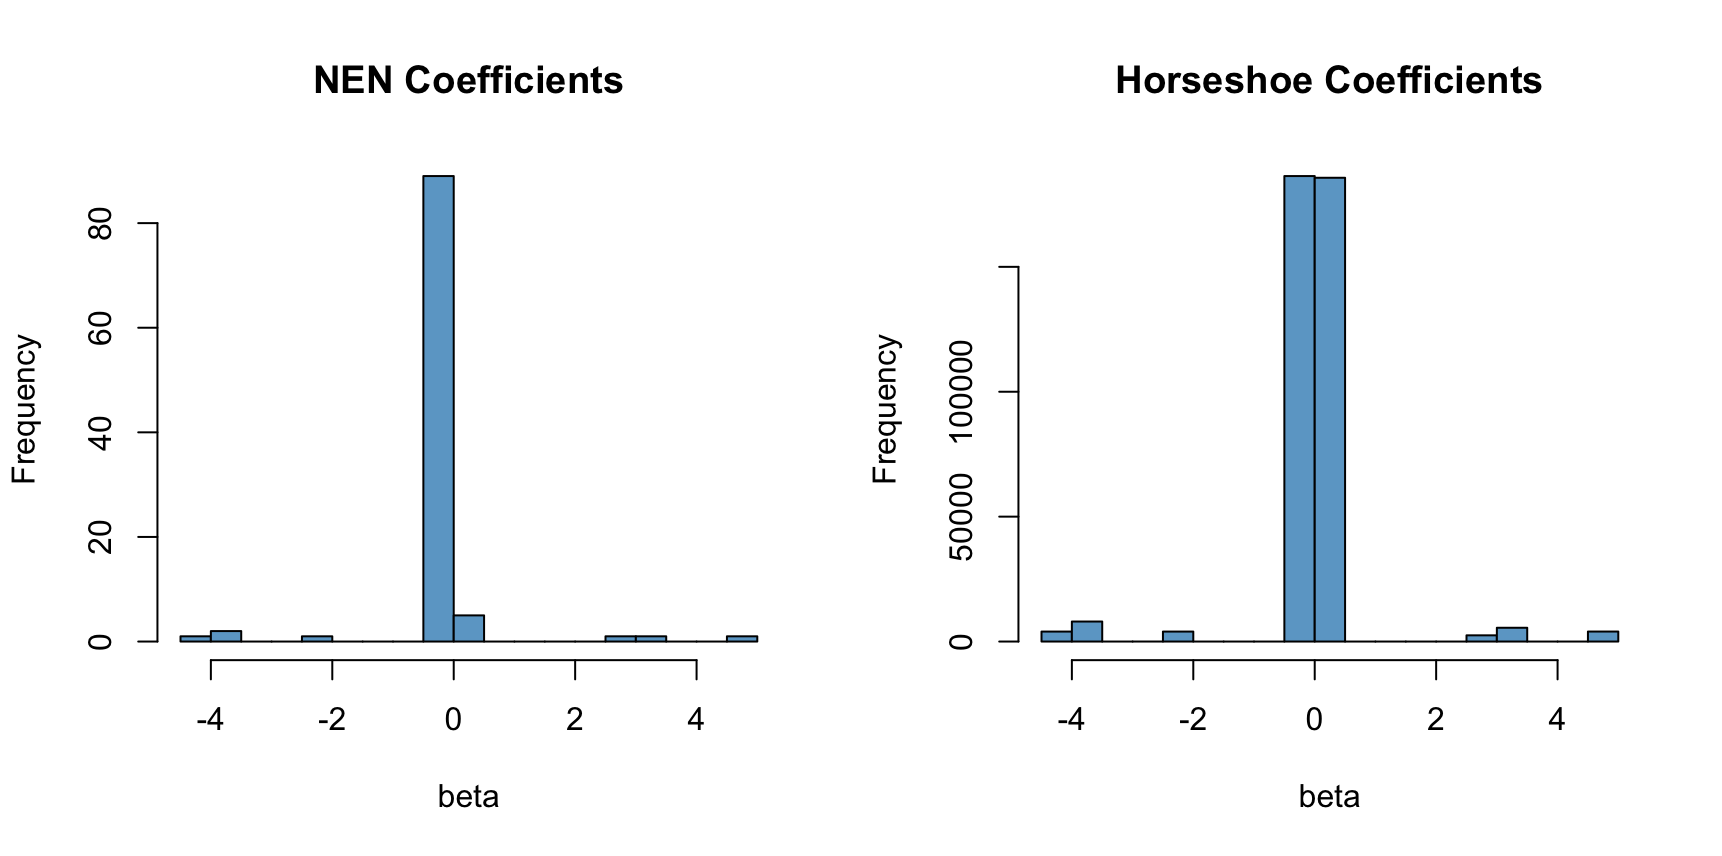
\includegraphics[width=0.6\textwidth]{Figures/simulate_betahat.png} 
\caption{\textbf{Estimated Coefficients} \\
Histograms displaying the estimated regression coefficients from NEN and Bayesian regression with a Horseshoe prior on simulated data.}
\label{fig:EN-lambda}
\end{figure} 



\begin{figure}[ht] %{figure*}[ht!]
\centering
\captionsetup{justification=centering, margin=-0.2cm}
\includegraphics[width=0.4\textwidth]{Figures/BC_lambda.png} 
\caption{\textbf{Breast Cancer Optimal Lambda} \\
Cross-validated errors over different values of $\lambda$ in the breast cancer data. Vertical lines indicate the most optimal values selected via cross validation.}
\label{fig:BC-lambda}
\end{figure} 

\end{document}
